\documentclass[10pt]{article}
\usepackage[polish]{babel}
\usepackage[utf8]{inputenc}
\usepackage[T1]{fontenc}
\usepackage{amsmath}
\usepackage{amsfonts}
\usepackage{amssymb}
\usepackage[version=4]{mhchem}
\usepackage{stmaryrd}
\usepackage{graphicx}
\usepackage[export]{adjustbox}
\graphicspath{ {./images/} }

\title{LIGA MATEMATYCZNA \\
 im. Zdzisława Matuskiego \\
 GRUDZIEŃ 2016 \\
 SZKOEA PONADGIMNAZJALNA }

\author{}
\date{}


\begin{document}
\maketitle
\section*{ZADANIE 1.}
Na bokach \(A C\) i \(B C\) trójkąta \(A B C\) zbudowano równoległoboki \(A C D E\) oraz \(B F G C\) tak, jak na rysunku. Punkty \(K\) i \(L\) są odpowiednio środkami odcinków \(E G\) i \(D F\). Oblicz \(\frac{|K L|}{|A B|}\).\\
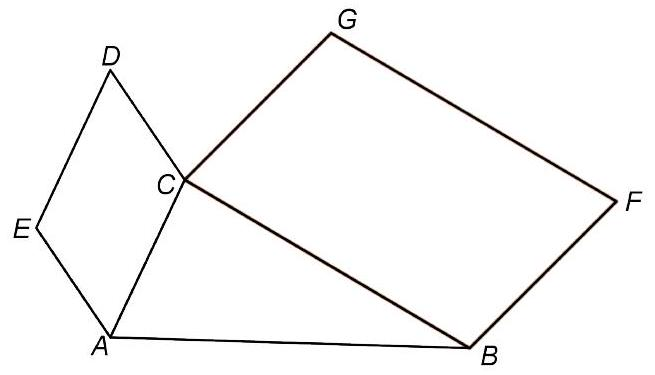
\includegraphics[max width=\textwidth, center]{2024_11_21_e2a822c97454b65cf5e4g-1}

\section*{ZADANIE 2.}
Znajdź wszystkie pary \((x, y)\) liczb całkowitych spełniające równanie

\[
x^{4}=y^{4}+1223334444
\]

\section*{ZADANIE 3.}
Na każdej ścianie sześcianu napisano pewną dodatnią liczbę całkowitą. Następnie w każdym wierzchołku sześcianu umieszczono liczbę, która jest równa iloczynowi liczb znajdujących się na ściankach, do których ten wierzchołek należy. Oblicz sumę liczb znajdujących się na wszystkich ścianach wiedząc, że suma liczb umieszczonych w wierzchołkach jest równa 70.

\section*{ZADANIE 4.}
Suma pewnych dziewięciu liczb jest równa 90 . Wykaż, że wśród nich są takie cztery, których suma jest równa co najmniej 40.

\section*{ZADANIE 5.}
Rozwiąż układ równań

\[
\left\{\begin{array}{l}
x^{3}-y^{3}=26 \\
x^{2} y-x y^{2}=6
\end{array}\right.
\]


\end{document}